\usetikzlibrary{arrows.meta,calc}
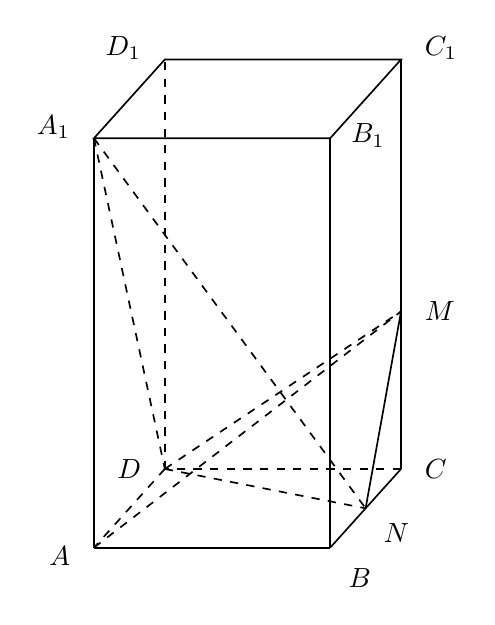
\begin{tikzpicture}[x=1cm,y=1cm,font=\normalsize,line width=.6pt]
% bottom face
\coordinate (A) at (0,0);
\coordinate (B) at (3,0);
\coordinate (C) at (3.9,1.0);
\coordinate (D) at (0.9,1.0);
% top face
\coordinate (A1) at (0,5.2);
\coordinate (B1) at (3,5.2);
\coordinate (C1) at (3.9,6.2);
\coordinate (D1) at (0.9,6.2);
% N on BC midpoint, M on CC1
\coordinate (N) at (3.45,0.5);
\coordinate (M) at (3.9,3.0);
% vertical edges
\draw[solid] (A) -- (A1);
\draw[solid] (B) -- (B1);
\draw[solid] (C) -- (C1);
\draw[dashed] (D) -- (D1);
% top face
\draw[solid] (A1) -- (B1) -- (C1) -- (D1) -- cycle;
% bottom face: front solid, back dashed
\draw[solid] (A) -- (B);
\draw[solid] (B) -- (C);
\draw[dashed] (C) -- (D);
\draw[dashed] (D) -- (A);
% bottom diagonals through D
\draw[dashed] (D) -- (N);

% interior diagonals
\draw[dashed] (A1) -- (D);
\draw[dashed] (A1) -- (N);
\draw[dashed] (A) -- (M);
\draw[dashed] (D) -- (M);
\draw[solid] (M) -- (N);
% M-C solid part of right edge already drawn; emphasize M point
% labels with clearance
\node[left,xshift=-5pt,yshift=-3pt] at (A) {$A$};
\node[below right,xshift=3pt,yshift=-4pt] at (B) {$B$};
\node[right,xshift=5pt] at (C) {$C$};
\node[left,xshift=-5pt] at (D) {$D$};
\node[left,xshift=-5pt,yshift=4pt] at (A1) {$A_{1}$};
\node[right,xshift=4pt,yshift=1pt] at (B1) {$B_{1}$};
\node[right,xshift=5pt,yshift=4pt] at (C1) {$C_{1}$};
\node[left,xshift=-5pt,yshift=4pt] at (D1) {$D_{1}$};
\node[below right,xshift=3pt,yshift=-2pt] at (N) {$N$};
\node[right,xshift=5pt] at (M) {$M$};
\end{tikzpicture}
